\section{Moving boundaries and the chordal limit}\label{sec:moving}

We now pass from the fixed polygon tests of
Theorem~\ref{thm:fixed-polygon} to the domains left by a growing strand.
There are two distinct tasks.  First, the four-change formula must hold
uniformly at suitably localized stopping times.  Second, the curves
must be compact in a topology that retains their entire time order.
The first task will supply bounded martingales; the second will justify
identifying both the driving process and the complete limiting curve.
Theorem~\ref{thm:moving-crossing} extends the fixed-polygon formula,
and Proposition~\ref{prop:slit-test} applies it to stopped histories.
Independently, Theorem~\ref{thm:c2} obtains curve compactness from
Theorem~\ref{thm:actual-disk} and the drawing and erosion geometry;
it does not use the stopped four-change formula.
These inputs combine in Proposition~\ref{prop:driver}, where the
mesh limit is taken before the inserted boundary interval shrinks.
The final proof identifies the full oriented curve, including its target.

Throughout this section, $q\in(0,1)$ is fixed and
\[
 d=\sqrt q=2\cos\lambda,\qquad
 \rho=\lambda/\pi\in(1/3,1/2),\qquad h=1-2\rho>0.
\]
All physical domains considered below lie in a common bounded set.
Boundary points, slots, and arcs of a cut disk always mean their
\emph{incidences} on that disk.  Coincidence of their planar images
does not identify them.

Retain the functions furnished by Theorem~\ref{thm:fixed-polygon}:
\begin{equation}\label{chordal:functions}
 f(\chi)=\frac{I_C(\chi)}{I_B(\chi)+I_C(\chi)},\qquad
 g(\chi)=\frac{f(\chi)}{f(\chi)+d(1-f(\chi))},
 \quad 0<\chi<1,
\end{equation}
where
\begin{align*}
 I_B(\chi)&=\int_\chi^1
 u^{\rho-1}(u-\chi)^{\rho-1}(1-u)^{1-3\rho}\,\dd u,\\
 I_C(\chi)&=\int_1^\infty
 u^{\rho-1}(u-\chi)^{\rho-1}(u-1)^{1-3\rho}\,\dd u.
\end{align*}
Here $f$ is the open-change pairing probability and $g$ is the
connection probability with the two tested-color electrodes wired
separately.  We use the cross-ratio convention for which a shrinking
electrode away from the other electrode has $\chi\downarrow0$.
In particular, $f(1-\chi)=1-f(\chi)$.

\subsection{Small accesses in normalized disks}

A \emph{thick normalization} of a disk $T$ is a conformal map
$\phi:T\to\D$ with $\phi(z)=0$, where $B(z,r_0)\subset T$ for a
fixed $r_0>0$.  Rotations may be fixed or extracted along a subsequence.
The disks here may have the cut-triangle boundary cells of
Section~\ref{sec:disks}; their interiors embed injectively in the plane.

\begin{lemma}[Uniform access estimates]\label{chordal:access}
Consider disks in a common bounded part of the plane with thick
normalizations $\phi_n$, and write $F_n=\phi_n^{-1}$.
\begin{enumerate}[label=(\roman*)]
\item A path in the closed disk of physical diameter $o(1)$ has
chart diameter $o(1)$ uniformly, provided boundary portions are
interpreted by interior approximation in their specified incidences.
\item A subsequence of $F_n$ converges on compact subsets of $\D$
to an injective nonconstant map $F$.  For an angular interval of
length $\ell$ and $0<\eta<1/4$, there is a radial segment in that
interval whose image from radius $1-\eta$ to the boundary has length
at most $C\sqrt{\eta/\ell}$, with $C$ uniform in $n$.
\item For the fixed limiting map,
\begin{equation}\label{chordal:derivative-tail}
 \sup_{|w|=1-\eta}\eta |F'(w)|\longrightarrow0
 \quad\text{as }\eta\downarrow0.
\end{equation}
\end{enumerate}
\end{lemma}

\begin{proof}
For (i), first keep the physical path a fixed positive distance from
the normalization point.  A Brownian motion started there hits a
set of diameter $\varepsilon$ before leaving a common enclosing ball
with probability tending uniformly to zero as $\varepsilon\downarrow0$;
the comparison with concentric round annuli gives, for example, a
constant times $1/\log(1/\varepsilon)$ after fixing the inner
clearance.  Conformal invariance gives the same conclusion for its
image, for Brownian motion started at $0$ in $\D$.

On the other hand, a connected path in $\D$ of diameter at least
$e>0$ has hitting probability bounded below by a positive constant
depending only on $e$.  If it reaches $\{|w|\le1-e/8\}$, take a
subcontinuum extending a fixed smaller distance from such a point;
the usual Brownian annulus estimate, or an encircling Brownian loop,
gives the lower bound.  Otherwise the path lies in the outer band.
Its radial variation is at most $e/8$, so its diameter lower bound
gives an angular variation bounded below in terms of $e$.  Choose a
width $\alpha_e\in(0,\pi)$ below that variation.  A first and last
level selection in a continuous angular lift gives a subpath joining
the radial sides of
\[
 \{1-e/8\le |w|\le1,\quad \theta_0\le\arg w\le\theta_0+\alpha_e\}
\]
and staying in that set.  Use the polar rectangle with the same
angular sides and inner radius $1-e/4$.  An entrance disk can be
chosen compactly inside its lower portion, below radius $1-e/8$ and
away from the radial sides.  Brownian motion from $0$ reaches that
disk before leaving $\D$ with probability bounded below in terms of
$e$.  From the disk, its first exit from the polar rectangle is
through the middle of the outer side with another uniformly positive
probability.  Such a confined trajectory must cross the spanning
subpath; an earlier hit already counts.  Boundary paths are obtained
by limits of interior paths.
Near the normalization point, interior distortion gives (i) directly.
This argument concerns a connected access: it makes no assertion
about two nearby points on different banks of a slit.

Boundedness gives normality of $F_n$.  The derivative at $0$ is
bounded below by the fixed physical disk, so a limiting map is
nonconstant; the limit of univalent maps is then univalent.  Since
the interiors are injectively embedded,
\[
 \int_{\D}|F_n'(w)|^2\,\dd\operatorname{area}(w)\le C.
\]
Cauchy--Schwarz along radial segments, followed by integration over
the angular window, proves (ii), since the radius is bounded below
on the indicated outer band.  Finally, the mean-value bound for
$|F'|^2$ in a disk of radius comparable to $\eta$ centered at
$|w|=1-\eta$ bounds $\eta^2|F'(w)|^2$ by a constant times the area
integral over an outer annulus.  That integral tends to zero, proving
\eqref{chordal:derivative-tail} uniformly on the circle.
\end{proof}

\subsection{The two-terminal test in a varying disk}

\begin{theorem}[Moving two-terminal crossing formula]
\label{thm:moving-crossing}
Let $T_n$ be tiled disks of the class in
Theorem~\ref{thm:pure-disk}, with mesh tending to zero, thick
normalizations, and a common bounded physical range.  In one color
wire separately all the slots of two disjoint boundary intervals
$A_n,B_n$, and impose no other ties.  Suppose the four interval
endpoints converge in chart coordinates to four distinct points in
their prescribed cyclic order.  If $\chi$ is their ordered
cross-ratio, then
\[
 \PP_{T_n}(A_n\leftrightarrow B_n)\longrightarrow g(\chi).
\]
The statement holds for either color, including cut-triangle cells
and repeated physical boundary locations with distinct incidences.
Equivalently, the error is uniform over sequences with fixed
thickness and fixed positive chart separation of the four endpoints.
\end{theorem}

The following construction supplies the uniformity needed in this
theorem.  It is important that it gives a short access from every
vertex of the auxiliary cut, not only from the cut's two ends.

\begin{lemma}[Inset cuts with short seams]\label{chordal:seams}
After passing to a subsequence as in Lemma~\ref{chordal:access}, fix
an angular trimming margin $\beta>0$ inside both electrode intervals
and a target tolerance $\varepsilon>0$.  One can first choose an inset
$\eta>0$, and then a sufficiently small precision $\zeta>0$ and a
fixed simple rational orthogonal polygon $K$ in tile coordinates.
Its closure is compactly contained in $F(\D)$, and it has a boundary
homeomorphism $k:\R/(2\pi\Z)\to\partial K$ tracing once in the prescribed
order with
\[
 \sup_\theta\left|F^{-1}(k(\theta))-(1-\eta)e^{\ii\theta}\right|
 \le \zeta\eta.
\]
Let $\tau_n$ be the current tile-coordinate mesh.  Choose a fixed
integer $M_K$ meeting the compatible-mesh requirements of the
fixed-polygon experiment, let $m_n\in M_K\N$ be nearest to
$\tau_n^{-1}$, and put $s_n=m_n\tau_n$.  A representative tile-grid
origin $o_n=O(\tau_n)$ can be chosen with the required color parity.
The exact whole-tile polygons
\[
 K_n=o_n+s_nK
\]
lie in $T_n$ for all sufficiently large $n$ and have the following
properties.
\begin{enumerate}[label=(\roman*)]
\item Two prescribed portions of $\partial K_n$ approximate the
trimmed electrode arcs in their boundary order.  Their endpoint marks
are eligible boundary gaps within $O(\tau_n)$ of fixed marks in flat
side interiors of $K$, transported by the displayed similarity.
\item For each electrode there is a proper simple tile-edge crosscut
$S_n$ following its prescribed portion of $\partial K_n$, extending
past that portion at both ends, and ending on the true electrode.
It cuts off an outer pocket whose boundary interval lies entirely
inside that electrode.  The two cuts and pockets are disjoint.
\item Every off-boundary vertex $z$ of $S_n$ has a simple tile-edge
seam to the true electrode inside the closed pocket, interior to
$T_n$ except at its final point.  Select one such seam $\gamma_{n,z}$
for each vertex of each cut, and let
\[
 \sigma_{n,\beta,\eta,\zeta}
 =\max_{\substack{\text{the two cuts}\\
                   z\text{ an off-boundary cut vertex}}}
       \operatorname{diam}(\gamma_{n,z}),
 \qquad \max\varnothing:=0.
\]
The choices can be made so that
$\limsup_{n\to\infty}\sigma_{n,\beta,\eta,\zeta}<\varepsilon$.
\item All these paths stay in the corresponding electrode sector,
with a positive angular submargin depending on $\beta$.
\end{enumerate}
The electrode cross-ratio of $K$ can at the same time be made within
$\varepsilon$ of that of the trimmed arcs.  For each choice of
$\beta,\varepsilon$, the inset is chosen first, the precision and
polygon next, and the mesh limit last.  In particular $K$ and $M_K$
are fixed during their mesh limit.
\end{lemma}

\begin{proof}
For fixed $\eta$, the image of the inset circle is an analytic Jordan
curve.  Cover it by short segments in disjoint narrow corridors and
replace them by sufficiently fine rational tile-coordinate
staircases.  Join consecutive staircases simply in disjoint small
vertex neighborhoods.  This yields a parametrized approximation of
the curve, including across the specified electrode positions; move
the marks into flat side interiors.  Uniform convergence to this
fixed analytic curve gives convergence of the normalized boundary
maps and hence of the cross-ratios.  The approximation can be chosen
with the stated chart error and boundary order.

We choose the copies $K_n$ to meet the compatible-mesh requirement
exactly.  Take $M_K$ to clear the tile-coordinate vertex denominators
and any fixed grid or parity requirements of the experiment in
Theorem~\ref{thm:fixed-polygon}.  Then
\[
 |s_n-1|\le \frac{M_K}{2}\tau_n,\qquad
 \sup_{z\in\overline K}|o_n+(s_n-1)z|=O_{K,M_K}(\tau_n).
\]
Every vertex of $K_n=o_n+s_nK$ is a vertex of the current tile grid.
The similarity $z\mapsto(z-o_n)/s_n$ sends its full tile graph exactly
to the fixed polygon $K$ at mesh $1/m_n$, with the ideal side lines
unchanged.  Only its marked gaps are rounded, by $O(1/m_n)$ in that
experiment.  The allowed color designation is transported by the
same map.

For containment, $\overline K$ is compactly contained in $F(\D)$.
If $d_K$ is its distance from $\C\setminus F(\D)$, compact kernel
convergence puts the closed $d_K/2$ neighborhood of $\overline K$
in $T_n$ for large $n$.  The displayed displacement is eventually
less than $d_K/3$, so $K_n$ remains in the uncut bulk with positive
clearance.  On that fixed compact neighborhood the maps
$F_n^{-1}$ converge uniformly to $F^{-1}$.  Thus the boundaries of
$K_n$ follow the inset circle in their current charts, with the
prescribed error relative to the fixed $\eta$ once the mesh is fine.
The similarities preserve the parametrized boundary order and the
short-subarc control of the polygonization.  The integer $M_K$ may
depend on this fixed polygon; the original mesh sequence remains
arbitrary.

Choose two angular windows between each trimmed interval and its
true endpoints, with spare margins.  Lemma~\ref{chordal:access}(ii)
gives short radial exits in these windows, starting just below
$1-2\eta$.  Follow them through consecutive tiles and then by
tile-edge paths to boundary vertices within one cell of their exits.
The two tile sides of a cut triangle also connect its corners.
Stop on the first true boundary hit and trim back to the last
$K_n$-exit before it.  Loop erasure and mesh rounding change chart
positions by $o(1)$, by Lemma~\ref{chordal:access}(i).  The two paths
therefore remain disjoint and in their separate windows.  Joining
them along the intervening arc of $\partial K_n$ gives the cut and
its pocket; boundary order locates the pocket inside the electrode.

For the assertion at every cut vertex, choose $C(\eta)\uparrow\infty$
so slowly that $C\eta\to0$ and every inset-circle arc of angular
width $O(C\eta)$ has image diameter $o(1)$.  This is possible by
\eqref{chordal:derivative-tail}.  Rounding is done after the inset
and polygon are fixed.  At fixed $\eta$, first choose $\zeta$ so
the polygon chart error $\zeta\eta$ is as small a fraction of
$\eta$ as needed, and then take the mesh fine enough to make the
tail-rounding and current-chart errors smaller still.  A vertex on
a tail can follow that tail.  A vertex on
the inset portion within angular distance $O(C\eta)$ of a tail can
first follow the short boundary arc to it.  Otherwise choose an
angular window of width comparable to $C\eta$ nearby and clear of
the two tail windows.  It contains an outward ray of physical
length $O(C^{-1/2})$ from radius $1-2\eta$ (or $1-3\eta$).
Round this ray at sufficiently fine mesh, trim it at its last
appropriate cut hit, and join to that hit along the short cut arc.
It reaches the true boundary between the two tails.  Erasing loops
gives the required seam in the pocket.  Parametrized polygonization
prevents a long backtrack along the inset circle.  The angular
submargins remain fixed; by Lemma~\ref{chordal:access}(i), small
physical approaches within the disk preserve them as well.

For fixed $\beta$, the terminal radial lengths and the short inset
arc diameters just obtained tend to zero as $\eta\downarrow0$.
Choose $\eta$ to make those contributions smaller than the desired
tolerance.  At that fixed inset choose the parametrized polygonization
fine enough that its short-subarc errors and its cross-ratio error
are smaller still.  Taking the mesh limit with this polygon fixed
then removes the path-rounding and chart-convergence errors.  This
gives the stated bound on the maximal selected seam diameter and
the simultaneous cross-ratio approximation.
\end{proof}

\begin{lemma}[The cost of moving an electrode]
\label{chordal:electrode-update}
In the construction of Lemma~\ref{chordal:seams}, let
$\Delta^{(1)}_{n,\beta,\eta,\zeta}$ be the increase in the
two-terminal connection probability when all tested-color vertices
of the first cut are added to its true electrode.  Define
$\Delta^{(2)}_{n,\beta,\eta,\zeta}$ similarly for the second cut
after the first pocket has been factored out.  There are $c,C>0$
and a fixed physical radius $r_\beta>0$ such that
\[
 0\le \Delta^{(j)}_{n,\beta,\eta,\zeta}
 \le C\left(
   \frac{\tau_n+\sigma_{n,\beta,\eta,\zeta}}{r_\beta}
       \right)^c,\qquad j=1,2.
\]
The notation $r_\beta$ suppresses its dependence on the fixed
thickness, common physical bound, and endpoint-separation data.
If $e_{n,\beta,\eta,\zeta}$ is the sum of the two right-hand bounds,
then for every $\varepsilon>0$ the inset and then the precision and
polygon can be chosen so that
$\limsup_{n\to\infty}e_{n,\beta,\eta,\zeta}<\varepsilon$.
Each polygon is fixed during its mesh limit.  The original FK
parameter is unchanged.
\end{lemma}

\begin{proof}
Write $p_{\rm old}$ and $p_{\rm new}$ for the connection probabilities
before and after one electrode update.  In the old law, let
$p_{\rm hit}$ be the probability that the opposite terminal reaches
the union of the true electrode and its cut.  The two finite
comparisons give
\[
 p_{\rm old}\le p_{\rm new}\le p_{\rm hit}:
\]
the first inequality is terminal enlargement in
Lemma~\ref{pressure:network-monotonicity}, and the second is
Lemma~\ref{pressure:general-no-hit}.  We prove that, conditional
on each search leaf exposing a witness of the hit event, failure to
reach the true electrode has probability at most the claimed error.  Averaging will
then bound $p_{\rm hit}-p_{\rm old}$, and hence the update cost.

\paragraph{Expose a witness with an uninspected side.}
Up to its first hit of the target union, a connection from the opposite
terminal is an actual open path,
with no jumps through the target wire.  It lies in the disk $R$ on
the outside-of-pocket side of $S_n$, and targets the whole boundary
interval $W$ consisting of the cut and exposed portions of the
original electrode.  A tile-edge cut is crossed at a corner vertex.
If the other electrode has already been updated, its pocket factors
through its one wire and is first removed.  For all separation
statements one may still use the original chart of $T_n$.

Search from the left boundary interval of $R$ for actual
complementary-color paths, without following identifications used
only in the weight.  Seed its exterior complementary face, query a
bond only from a reached complementary face, and enter an interior
face only across a tested-closed physical bond.
The left and right search intervals run between
the extreme tested slots of the opposite terminal and $W$.
Nonarrival at the right interval is exactly the existence of the
tested crossing, by the disk path/cut alternative.  Equivalently,
one can prolong fictitious spokes from the two target intervals
just outside the disk and search for a separating complementary
crossing between them.  These spokes change neither the law nor
the actual edge event.

On exhaustion the inspected tested-open edges contain a crossing:
turning every uninspected bond complementary-open would still leave
the search exhausted.  Choose a simple measured witness $P$, trimmed
after its last visit to the start interval and before its first
subsequent target reach.  Its interior avoids
$S_n$.  The interiors of edges strictly on its right in $R$ are
uninspected, since a complementary search from the left cannot
cross the blocker.  This remains true for a boundary diagonal of a
half cell: bend it infinitesimally into the cell so that it crosses
the complementary spoke before the degree-one virtual endpoint,
and flatten it back after making the separation argument.  No edge
on the unsearched side is thereby queried.

\paragraph{The seam bounds a protected disk.}
Figure~\ref{fig:short-seam} illustrates the next construction.
If $P$ already touches the true electrode, the desired connection
has occurred.  Otherwise its final point $z$ lies strictly on $S_n$.
Use the short seam $\gamma$ from $z$ furnished by
Lemma~\ref{chordal:seams}.  Starting from $P$'s initial point, follow
the right outer boundary arc to the terminal point of $\gamma$.
Take the subarc $L_*$ beginning at the last hit of this arc by $P$,
and the tail of $P$ following that hit.  This tail, $L_*$, and
$\gamma$ enclose a Jordan disk on the right.  Indeed the tail has
no subsequent contact with $L_*$ and has no contact with the seam
before $z$, since the seam is in the pocket.  Contacts with other
outer-boundary portions are interpreted on the abstract disk.

The portion of this disk in $R$ is on the uninspected side of $P$.
To check the side even when $\gamma$ follows $S_n$ initially, replace
the boundary portion inside the closed pocket by its arc on $S_n$.
This deformation changes no winding number in $\operatorname{int}R$.
The resulting loop is exactly the right-side loop of the blocker,
using the right outer boundary up to its first cut hit.  The search
starts are on the other side.  Earlier portions of $P$ cannot enter
the loop without crossing its tail or the cut; the remaining outer
arc is a domain boundary.  The pocket itself was never inspected.

Beginning at the seam, $L_*$ belongs to the true electrode for a
fixed angular margin: a measured contact in that margin would
already give the desired connection.  Split $L_*$ at a chart
position between the seam's submargin and the end of the electrode.
The remainder, up to the contact with $P$, is chart-far from the
seam.  This remains so if the opposite electrode has previously
been moved.  Lemma~\ref{chordal:access}(i) therefore supplies a
small fixed physical radius, uniform in the histories, such that
no access of that diameter from the seam reaches the far interval.
Choose a smaller such radius and call it $r_\beta$.  If
$\tau_n+\sigma_{n,\beta,\eta,\zeta}$ is not a sufficiently small
fraction of $r_\beta$, the claimed bound is trivial after enlarging
$C$, since a probability increase is at most one.  Work in the
remaining range.

At a tile-coordinate square level of this radius about $z$, choose
the first visible crosscut $J$ joining the $P$ flank to the
true-electrode flank and separating the seam from the far interval.
Here is a discrete way to make this choice.  Take the component
accessible from the seam before reaching that level, using a
slightly larger radius as a buffer.  Its closure misses the far
interval.  The frontier facing that interval contains a connected
level path between the two flanks, by the disk path/cut alternative;
trim it between its last and first opposite flank contacts.
Integer square levels follow tile edges and meet a diagonal side
only at a corner.  If the frontier has a pinch, trace the boundary
of the near reachable cells in disk incidences and make the same
trimming.  Thus $J$ is a proper crosscut with the required corner
contacts.  Its $P$-contact is still chart-near the seam.

The new $P$ flank is cut along measured whole diagonals.  It does
not cut a virtual-slot spoke: a simple actual path can use such a
spoke only at its first or last edge; the first is chart-far at
the opposite terminal, and the first hit $z$ of a tile-edge cut is
a corner, not the virtual midpoint.  Hence no quarter cells are
needed.  Between $J$ and the seam, retain the half cell on the
uninspected side of each measured diagonal.  Its tested endpoints
are already tied by $P$, so resampling that diagonal at the ordinary
odds changes no network event.  The opposite-color virtual spoke
only dangles.  All other interior bonds are uninspected.

\paragraph{Failure forces an actual opposite-color passage.}
Conditional on compatible outside states, the two tested flanks are
fully wired, one by the actual measured path and the other by the
true electrode.  Additional ties are planar.  Draw consecutive
links of each full flank wire narrowly outside its slots before
drawing the remaining links.  Euler duality and the disk path/cut
alternative show that failure of the flank connection requires an
\emph{actual} opposite-color passage from the seam to $J$.  Its
possible exterior identifications form a joint planar partition on
the two end cuts only: intermediate dual flank slots are free,
and the corner slots belong to the corresponding ends.  Measured
diagonal links are drawn outside the retained half cells, so this
argument uses the original disk order even at repeated contacts.

After rescaling from unit tile mesh, Theorem~\ref{thm:actual-disk}
bounds that conditional passage probability by
\[
 C\left(\frac{\tau_n+\operatorname{diam}\gamma}{r_\beta}\right)^c.
\]
The seam is contained in a ball of its physical diameter about $z$,
whereas $J$ is at a fixed positive radius comparable to $r_\beta$.
Only measured information selected the disk; the untouched cells
were not conditioned on failure of a connection.  Thus, with $a_n$
denoting the asserted error bound, averaging over the search leaves
on the hit event gives
\[
 0\le p_{\rm new}-p_{\rm old}
 \le p_{\rm hit}-p_{\rm old}
 \le a_n p_{\rm hit}\le a_n.
\]
The same argument applies to the second update after removing the
first pocket through its single wire.  The choice
statement in Lemma~\ref{chordal:seams}, with its seam tolerance chosen
in terms of the desired probability error and $r_\beta$, then makes
the upper limit of the sum smaller than any prescribed
$\varepsilon$.  This last choice sends the mesh to zero only after
the inset and polygon have been fixed.
\end{proof}

\begin{figure}[tbp]
\centering
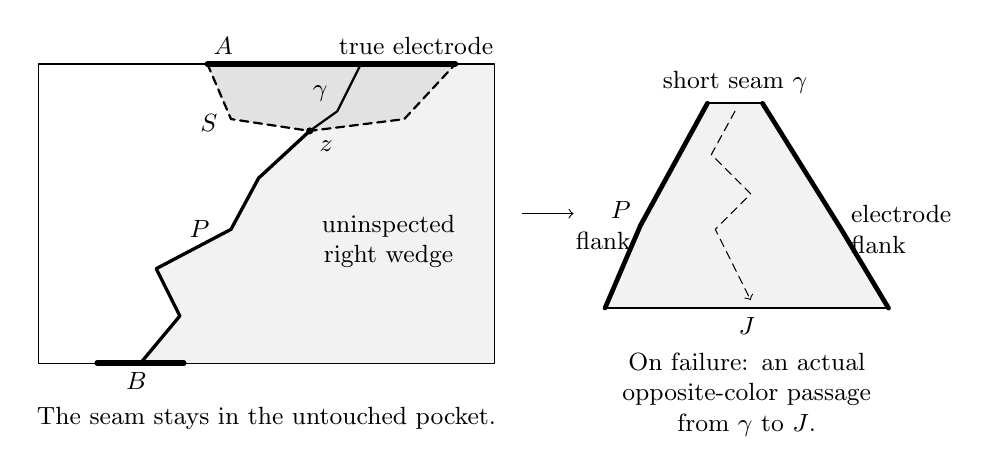
\begin{tikzpicture}[x=1cm,y=1cm,font=\small,line cap=round,line join=round]
  \path[fill=gray!10] (1.3,0) -- (1.8,.6) -- (1.5,1.2) -- (2.45,1.7)
    -- (2.8,2.35) -- (3.45,2.95) -- (4.1,3.8) -- (5.8,3.8) -- (5.8,0) -- cycle;
  \path[fill=gray!23] (2.15,3.8) -- (2.45,3.1) -- (3.45,2.95) -- (4.65,3.1) -- (5.3,3.8) -- cycle;
  \draw (0,0) rectangle (5.8,3.8);
  \draw[line width=2pt] (2.15,3.8) -- (5.3,3.8);
  \draw[line width=2pt] (.75,0) -- (1.85,0);
  \draw[densely dashed,thick] (2.15,3.8) -- (2.45,3.1) -- (3.45,2.95) -- (4.65,3.1) -- (5.3,3.8);
  \draw[line width=1.2pt] (1.3,0) -- (1.8,.6) -- (1.5,1.2) -- (2.45,1.7)
    -- (2.8,2.35) -- (3.45,2.95);
  \draw[thick] (3.45,2.95) -- (3.8,3.2) -- (4.1,3.8);
  \fill (3.45,2.95) circle (.045);
  \node[below right] at (3.45,2.95) {$z$};
  \node[left] at (2.3,1.7) {$P$};
  \node[above] at (2.35,3.8) {$A$};
  \node[below] at (1.25,0) {$B$};
  \node[left] at (2.4,3.05) {$S$};
  \node[left] at (3.8,3.42) {$\gamma$};
  \node[align=center] at (4.45,1.55) {uninspected\\right wedge};
  \node[above] at (4.8,3.8) {true electrode};
  \node[align=center] at (2.9,-.7) {The seam stays in the untouched pocket.};
  \draw[->] (6.15,1.9) -- (6.8,1.9);
  \path[fill=gray!10] (7.2,.7) -- (7.65,1.75) -- (8.5,3.3) -- (9.2,3.3)
    -- (10.2,1.7) -- (10.8,.7) -- cycle;
  \draw[line width=1.7pt] (7.2,.7) -- (7.65,1.75) -- (8.5,3.3);
  \draw[line width=1.7pt] (9.2,3.3) -- (10.2,1.7) -- (10.8,.7);
  \draw[thick] (8.5,3.3) -- (9.2,3.3);
  \draw[thick] (7.2,.7) -- (10.8,.7);
  \draw[densely dashed,->] (8.85,3.2) -- (8.55,2.65) -- (9.05,2.15) -- (8.6,1.7) -- (9.05,.8);
  \node[above] at (8.85,3.3) {short seam $\gamma$};
  \node[below] at (9,.7) {$J$};
  \node[left,align=right] at (7.65,1.75) {$P$\\flank};
  \node[right,align=left] at (10.2,1.7) {electrode\\flank};
  \node[align=center,text width=4.8cm] at (9,-.4)
    {On failure: an actual\\opposite-color passage\\from $\gamma$ to $J$.};
\end{tikzpicture}
\caption{Extending a moving electrode. Left: an actual extremal path $P$ first hits the inset cut $S$ at $z$; the small seam $\gamma$ reaches the true electrode through the untouched pocket. The tail after the last right-boundary hit, the seam, and the right outer boundary bound the protected wedge. Right: the subdisk between the seam and a farther cut $J$, drawn in abstract disk coordinates. Both flanks are wired in the tested color. Failure of their connection is an actual opposite-color hard passage with ties confined to its ends. The wedge is chosen from measured information; the future failure event is not used to condition its law.}
\label{fig:short-seam}
\end{figure}


\begin{proof}[Proof of Theorem~\ref{thm:moving-crossing}]
It suffices to prove the lower bound in each color.  In fact,
if $p$ is the separately wired probability in one color, Euler
duality gives the complementary separately wired probability
\begin{equation}\label{chordal:dual-map}
 H(p)=\frac{1-p}{1-(1-q)p}.
\end{equation}
The function $H$ is continuous and decreasing, and
$H(g(\chi))=g(1-\chi)$, using
$f(1-\chi)=1-f(\chi)$ and $q=d^2$.

Pass to any subsequence and then extract the limiting map in
Lemma~\ref{chordal:access}.  Fix a trimming margin $\beta$ and write
$\chi_\beta$ for the cross-ratio of the trimmed arcs.  Given
$\varepsilon>0$, choose the inset, then the precision and polygon,
as in Lemmas~\ref{chordal:seams} and~\ref{chordal:electrode-update},
so that the fixed polygon cross-ratio $\chi_K$ is within
$\varepsilon$ of $\chi_\beta$ and
$\limsup_n e_{n,\beta,\eta,\zeta}<\varepsilon$.
Moving both electrodes to the cuts costs at most
$e_{n,\beta,\eta,\zeta}$ in connection probability.  Each pocket factors
out through its one wire.  In the remaining disk release every
terminal link except those wiring the prescribed electrode
intervals of $K_n$; by the terminal assertion of
Lemma~\ref{pressure:network-monotonicity}, this does not increase the network probability.

Next remove the edges outside $K_n$ by cofacial peeling, which also
does not increase this particular two-terminal probability.  The geometric
justification matters here.  The two retained wire intervals are
exposed on the residual boundary and can be realized by exterior
chains.  An unwanted edge has a point outside the filled simple
polygon $K_n$, and hence an approach from an exterior gap avoiding
$K_n$.  Place an auxiliary connection-test edge across that gap
between representatives of the two terminals.  Peeling along the
approach makes each successive removed edge cofacial with the test.
The exterior chains abut $K_n$ and do not seal such a gap; their
thin realizations can be avoided.  Different gaps may use different
placements of the test edge, since after taking the chain odds to
infinity they test the same two terminals.  Isolated extra vertices
do not affect the probability.  The cofacial assertion of
Lemma~\ref{pressure:network-monotonicity} therefore gives
\[
 \PP_{T_n}(A_n\leftrightarrow B_n)
 \ge \PP_{K_n}(A'_n\leftrightarrow B'_n)
       -e_{n,\beta,\eta,\zeta}.
\]
For this fixed $K$, the exact similarity in
Lemma~\ref{chordal:seams} identifies the experiment on $K_n$ with
the compatible fixed-polygon experiment.  Theorem~\ref{thm:fixed-polygon}
therefore gives
$\PP_{K_n}(A'_n\leftrightarrow B'_n)\to g(\chi_K)$.
Taking the mesh liminf with this one polygon fixed gives
\[
 \liminf_n\PP_{T_n}(A_n\leftrightarrow B_n)
 \ge g(\chi_K)-\limsup_n e_{n,\beta,\eta,\zeta}
 \ge g(\chi_K)-\varepsilon.
\]
For fixed $\beta$, this construction is available for every
$\varepsilon>0$, and $|\chi_K-\chi_\beta|<\varepsilon$.
Continuity of $g$ therefore gives the lower bound
$g(\chi_\beta)$ as $\varepsilon\downarrow0$.  Each application
of the fixed-polygon theorem used one polygon held fixed during its
mesh limit; no uniformity over polygonizations is required.
Finally let $\beta\downarrow0$ and use continuity once more.
Apply the same argument in the other
color and use \eqref{chordal:dual-map} for the upper bound.
One-slot endpoint changes have vanishing chart size by
Lemma~\ref{chordal:access}, so are absorbed by the angular margins.
The sequential argument proves the asserted uniformity.
\end{proof}

\subsection{A drawing compatible with the finite law}

We specify the discrete representation before applying the moving
formula to a stopped interface.  No change to the finite law in
Theorem~\ref{thm:main} is made.

\begin{lemma}[A gapped simple drawing]\label{chordal:drawing}
At the initial drawing interface, let $D_\delta$ be the bounded
interior of a simple closed nearest-neighbor polygon in $\delta\Z^2$, and
let $a_\delta,b_\delta$ be distinct vertices of that polygon.
Use the full graph of vertices and edges in the closed polygon.
The wired arc is a closed boundary arc including both marked vertices.
Every graph edge is sampled in the law, and exactly the boundary edges of that arc are
declared open for the prescribed drawing.  For this graph and law
in Theorem~\ref{thm:main}, there is a tiled topological disk $V_\delta$
with injectively embedded interior and a rounded strand with the
following properties.  Below we write $V=V_\delta$ when the mesh is fixed.
\begin{enumerate}[label=(\roman*)]
\item The marked boundary tracing of $V$ is at distance $O(\delta)$
from that of the original polygon.  The rounded strand's actual
medial boundary endpoints $a_\delta^V,b_\delta^V$ are within
$O(\delta)$ of $a_\delta,b_\delta$, respectively.  Along a uniformly
convergent marked Jordan sequence, fix $z_*\in D$.  Eventually
$z_*\in V_\delta$, and the inverse disk maps
\[
 F_\delta:\D\longrightarrow V_\delta,\qquad
 F_\delta(0)=z_*,\qquad F_\delta'(0)>0
\]
converge uniformly on the closed disk to the correspondingly
normalized map $F:\D\to D$.  The preimages of
$a_\delta^V,b_\delta^V$ converge to those of $a,b$.
\item The rounded strand is simple, lies in $\operatorname{int}V$
except at its two endpoints, and matches the ordered local pieces
of the prescribed medial strand at curve distance $O(\delta)$.
It uses polygonal templates with uniformly nondegenerate angles
and gaps at least $c\delta$ between nonincident pieces, and between
the inner drawing and the wall except at endpoint transversals.
\item At a switch-revealing stop its unknown original edges have
the ordinary conditional FK law, with known open edges contracted
and known closed edges deleted.  Bank sites have access to the
corresponding side of the prefix within physical diameter $O(\delta)$.
Designated boundary slots have simultaneous short outward accesses
to their own intervals.
\item The same construction is available for four open changes.
Separate deterministic closure in a tested color changes the
conditional open pairing probability $p$ into
\begin{equation}\label{chordal:cap-odds}
 p\longmapsto\frac{p}{p+d(1-p)}.
\end{equation}
The drawings and normalization can be kept identical away from an
interval on which an extra pair of changes is inserted.
\end{enumerate}
All accesses and gaps refer to the appropriate disk sectors at slit
contacts; they do not pass through a wall to another incidence.
\end{lemma}

\begin{proof}
Use one full checkerboard tile for each graph edge, including its
exterior triangular tab when it is a boundary edge.  Within each
ordinary square, glue its four incident triangles across their
matching port sides.  Do not glue different exterior tabs along
their radial sides.  Simplicity of the initial polygon gives one
interior polygon fan at each boundary vertex.  A primal boundary
vertex retains that fan and the tabs at its two extreme edges.
Tile interiors
and glued-side interiors are disjoint under planar projection;
additional coincidences occur only on boundary incidences.
A concave fan can have full angle $2\pi$, in which case its extreme
sides form a slit rather than being identified.  The result is a
topological polygonal disk.  Its boundary follows the original
boundary with detours of diameter $O(\delta)$.

The assumed closed counterclockwise boundary parametrizations trace
once, are injective on $[0,1)$, and converge uniformly with their
marked cyclic parameters.  The compression below preserves this
tracing order and moves the boundary by $O(\delta)$.  Uniform
parametrized convergence to a simple Jordan boundary
implies uniform local connectedness of these boundary images:
nearby image points have nearby parameters, up to the short
detours, and are joined along a boundary segment of uniformly small
diameter.  Kernel convergence and the boundary extension criterion
then give uniform convergence of normalized inverse maps on the
closed disk.  The side-interior endpoint transversals are within
$O(\delta)$ of the marked polygon vertices.  Uniform convergence
of the boundary maps and injectivity of the limiting Jordan map
therefore give the claimed convergence of their preimages.
Repeated boundary incidences still use their own prime sectors.

Slightly compress the tile complex into $V$, leaving a thin collar
for the cap arcs and unmatched-port extensions; denote this
compression by $\sigma$.  Draw each switch by two disjoint simple
turn arcs toward the corresponding corners, avoiding both those
corners and the opposite boundary diagonal.  On a designated
interval use the local caps between successive visits of its color;
an unassigned slot is capped around between its two incident ports.
A designated slot has a short outward access between caps; the
outward access from an undesignated slot crosses just its surrounding
cap.  At a change leave the appropriate port unmatched and extend
it to a side-interior boundary point by an initially perpendicular
straight segment.  These are the only contacts of a chord with the wall.

Here the compression and arcs can be chosen from finitely many
polygonal templates.  Inset each boundary edge in a strip and each
vertex within its abstract fan, matching by a fixed subdivision of
the adjacent tiles, and leave $\sigma$ unchanged off an
$O(\delta)$ boundary neighborhood.  Fans have at most full angle
$2\pi$.  At coincident slit sides make the offsets on their
respective inset sides.  Ports lie away from side endpoints and
arcs meet there transversely.  There are only finitely many scaled
local configurations of fans, caps, changes, and switches, so the
choices give uniform positive gaps and angle bounds.  In particular,
an interior access of diameter $o(\delta)$ near a join can encounter
only its local incident pieces; it cannot confuse opposite slit
half-neighborhoods.  Every piece length and displacement is
$O(\delta)$.  The compression is used only for drawing, not as a
conformal map.

The positive loop identity follows directly in this representation.
Draw planar exterior trees for the separate tested wires and thicken
the open graph together with these trees.  If $\ell$ is its number
of perimeter components, Euler's formula gives
\[
 \ell=2k(A)+|A|+\text{a constant independent of }A.
\]
Consequently $d^\ell$ is proportional to
$q^{k(A)}d^{|A|}$, the finite FK weight.  This calculation uses only
$d>0$.  Conditional component counting gives the same statement
after revealing switches, with the induced contractions and deletions.

At an originally wired boundary edge, its endpoints were already
identified, so its sampled state is an independent loop variable
for weighting.  The exterior dual cap joins its inner continuations
in the same way in either state.  Declaring the edge open for the
prescribed drawing replaces a bounded-size cap detour and possibly
removes a microscopic closed loop.  On the free arc, the cap around
a primal singleton is the boundary turn beside the dual wired arc.
Match the remaining pieces in their occurrence order.  Simultaneous
parametrizations differ by $O(\delta)$, including at a medial point
visited with two different pairings; constant pieces are handled
by limits of increasing homeomorphisms.  This proves the drawing
claim in exactly the curve metric of Theorem~\ref{thm:main}.

Along a known bank, a revealed diagonal of that color connects its
two sites, and a turn around a site of that color stays at that site.
A cap stays at one site or follows consecutive sites of its designated
wire.  Thus each bank is attached to its original electrode and has
the claimed local accesses.  The two color accesses at a tile can
be drawn on their respective sides of the turn, simultaneously
with the designated slot accesses in the collar.

With four open changes there are two noncrossing pairings.  Under
separate tested-color closure, the connection alternative adds one
completed loop and its complement adds two.  Their full-sample
relative weights are therefore $d$ and $d^2$.  Conditioning that
full density on any history gives \eqref{chordal:cap-odds}; it is
not a limiting domain Markov assertion.  The density and its
reciprocal are bounded in terms of the fixed $q$.  In the two-change
case the pairing is forced and closure introduces no bias.
Insertion changes only the local caps and designations near the
new interval, so the rest of the drawing may be left unchanged.
\end{proof}

\subsection{Eroding a revealed prefix}

\begin{lemma}[Remaining tiled pieces]\label{chordal:erosion}
Stop the rounded strand at a local piece junction, with the states
of all encountered switches known but no unused next step specified.
Let $U$ be $V$ slit along its simple prefix.  There is a collection
of remaining tiled disks with cut-triangle cells such that:
\begin{enumerate}[label=(\roman*)]
\item Their compressed interiors are disjoint open subsets of $U$.
Every point outside these interiors, including their boundaries,
has a path of diameter $O(\delta)$ to the prime boundary of $U$
outside the piece interiors.
\item For a fixed color, the only interactions between pieces are
the original wires and the ties supplied by known banks.  A
non-dummy site with different remaining fan occurrences is already
tied to a known bank.  Every untied site has its complete remaining
incident fan in one piece.
\item On a half cell cut along a measured open diagonal, its color
endpoints are tied and the opposite-color virtual midpoint is free.
One may resample the half-cell state at the ordinary input odds
without changing unknown original-edge laws or terminal probabilities.
\end{enumerate}
These assertions also hold after advancing a stop by boundedly many
local pieces, with short accesses measured in the original stopped
disk.  New bank contacts from that advance access the old tip within
$O(\delta)$.
\end{lemma}

\begin{proof}
Use the uncompressed tile geometry to perform the following erosion.
For a visited turn remove the triangle on that side of the revealed
diagonal, namely the triangle containing the corner turned around.
If both turns have been visited, remove both triangles.  Retain a
remaining triangle as a cut-triangle cell and split every corner
into its remaining connected sectors.  The resulting pieces are
connected through their still glued sides.

Successive removed triangles connect through the crossed port sides
back to the beginning of the prefix on the exterior boundary.
Segments ending at a visited outer cap also connect to the exterior.
Thus there is no isolated removed component enclosing a hole.
More explicitly, in the complement of the regular open interior of
a retained component every removed cell is connected to the exterior
by such a chain; any other retained component adheres to these
chains or the outer boundary.  That complement is connected.
Splitting disconnected corner fans makes each retained component a
compact polygonal surface with simply connected interior and hence
a topological disk.  Its uncompressed interior remains injectively
embedded in the original grid.

Every previously crossed port, except possibly the current tip
junction, has both continuation triangles removed, or borders a cap
and a removed triangle.  Hence a compressed piece meets the measured
strand only at an exposed used port at the current end.  From a
removed triangle one can approach its visited turn on the relevant
side within that triangle; if another removed region is encountered
first, use its first boundary encounter.  A cut diagonal has the
same access through its removed triangle.  Collar points have the
corresponding cap or wall access.  This proves the first assertion
with the indicated disk incidence at contacts.

The bank-chain description in Lemma~\ref{chordal:drawing} shows
that a measured diagonal of the tested color is already contracted
to that bank's wire.  Its opposite-color midpoint is a new free
dummy slot.  The diagonal can therefore be sampled independently
as a loop at the ordinary odds.  From the opposite-color viewpoint
the spoke only dangles, and its opening odds after the component
factor are $v/q$, with input odds still $v$.  Integrating it out
does not change any other state or terminal event.  This explains
the half-cell convention without claiming a new drawing inside an
already measured cell.

If an ordinary color site has two disconnected remaining sectors,
some removed triangle at that corner has put the site on a known
bank.  Conversely an untied site has no such removed corner sector,
so its available incident fan is still connected in one piece.
The original weights conditioned on the history depend on unknown
edges only through component counts after contraction of known
open paths and the original wires.  Thus shared tied sites and
these wires exhaust all interactions between the pieces.

Finally, a bounded local advance removes only boundedly many
additional triangles or collar pieces, all adjacent to the old tip
or the portion just traversed.  Their exterior accesses run back
through these discarded strips to the old tip within $O(\delta)$.
No unrelated state need be queried.  The same assertions therefore
hold with accesses taken in the original stopped disk.
\end{proof}

\begin{proposition}[The localized stopped four-change test]
\label{prop:slit-test}
Fix $q\in(0,1)$ and $r_0,s_0,M>0$.  Let
$\mathcal H_\delta(r_0,s_0,M,q)$ consist of the following data:
a rounded four-open-change experiment from
Lemma~\ref{chordal:drawing} at mesh $\delta$ with $V\subset B(0,M)$;
a compatible history $\omega$ of its strand at a path-adapted
stopping time $\tau$,
from the original first mark, before completion and revealing only
encountered switches; and a point $z$ such that $B(z,r_0)\subset U$,
where $U$ is the remaining slit disk.  Require the tip and the three
remaining marked prime ends to have pairwise Euclidean distance at
least $s_0$ in a disk chart $\varphi_U:U\to\D$ with $\varphi_U(z)=0$.
The condition is independent of the chart's rotation.  If $E$ is
the tested-color pairing alternative and $\chi_U$ is the current
ordered cross-ratio, then
\begin{equation}\label{chordal:stopped-test}
 \varepsilon_{\rm stop}(\delta;r_0,s_0,M,q)
 :=\sup_{\mathcal H_\delta(r_0,s_0,M,q)}
 \left|
 \PP_{\rm open}(E\mid\mathcal F_\tau)(\omega)
       -f(\chi_U(\omega))
 \right|
 \longrightarrow0\qquad(\delta\downarrow0).
\end{equation}
An empty supremum is zero.  The class includes stops inside local pieces.
\end{proposition}

\begin{proof}
First restrict to junction stops.  If the stated supremum did not
tend to zero for that subclass, choose $\delta_n\downarrow0$ and
data from the class whose errors stay bounded away from zero.
Write $U_n$ for their slit disks and normalize their disk charts at
the chosen basepoints.  Pass to a subsequence on which the four
marked chart positions converge; their limits remain distinct by
the fixed separation.  We prove convergence along this sequence.
The required reduction has three parts: find the one remaining tiled
disk carrying the macroscopic chart, match its boundary incidences to
the stopped chart, and identify its conditional law as a two-terminal
law up to arbitrarily small angular margins.

\paragraph{The two terminals remain distinct.}
Use separate closure in one color.
There is no contact of its known bank with the other electrode of
that color under the stated localization.  Indeed, until a first
such contact, the bank is attached to its starting electrode.
At a purported contact the site has simultaneous short accesses
to that bank side and to the distinct original electrode, by
Lemma~\ref{chordal:drawing}.  Their concatenation is a connected
physical access of diameter $O(\delta)$ with chart endpoints in
separated intervals, contradicting Lemma~\ref{chordal:access}.
A visit to another electrode through a cap has the same property.
Thus the two terminal wires remain distinct.

\paragraph{One remaining piece carries the disk chart.}
Erode the history as in Lemma~\ref{chordal:erosion}.  In the
$U_n$ chart every fixed compact subset of $\D$ eventually belongs
to a single compressed piece, denoted $T_n$.  Interior distortion
at the thick basepoint gives a fixed positive physical clearance
for such a compact set, whereas all removed cells and boundary
deformations are within $O(\delta)$ of a wall or queried tile.
The short accesses from the exterior of the pieces have chart
diameter $o(1)$.

Every other piece has chart diameter $o(1)$, uniformly, including
its boundary accesses.  Otherwise, since the other pieces avoid
every fixed chart compactum, one contains a path spanning a polar
rectangle of fixed angular width in an outer annulus.  Select a
subpath joining its radial sides and staying between them.  The
middle radius from the core of $T_n$ must meet this subpath before
reaching the unit circle.  Its first exit from $T_n$ occurs earlier,
on the inner side of the spanning subpath.  From that exit, the
short exterior access supplied by erosion reaches the unit circle
without entering any piece interior.  Its chart diameter is $o(1)$,
so it stays between the two radial sides.  It must therefore cross
the spanning subpath to reach the outer boundary, contradicting
that subpath's location in another piece interior.
This proves the assertion without assuming physical boundary
regularity of the stopped domains.

\paragraph{Match the boundary incidences, not only the kernels.}
The normalized chart of the \emph{uncompressed} tiled disk $T_n$
agrees, also on its boundary incidences, to $o(1)$ with the ambient
$U_n$ chart of its compressed image.  We give the details because
interior kernel convergence alone would not suffice here.
On chart compacta the erosion and compression do nothing.  Thus
the pointed kernels agree and the normalized charts match in the
interior.  Conversely, any fixed cleared path with spare-width
neighborhoods in the main piece remains in the slit-disk kernel:
its $O(\delta)$-displaced embedded neighborhoods surround a
slightly smaller tube, by injectivity and degree.  These observations
give the two-sided interior kernel assertion.

For boundary matching, choose finitely many well-spaced marker
angles in the piece chart.  Close to each marker select a ray with
a short physical terminal segment from radius $1-\eta$ to the
piece boundary, using Lemma~\ref{chordal:access}(ii).  Avoid the
finitely many vertex coincidences.  Continue its compressed endpoint
to the boundary of $U_n$ by the short exterior access, trimmed not
to reenter the piece.  Interior matching and
Lemma~\ref{chordal:access}(i) keep each combined access in a small
angular neighborhood of its marker in the $U_n$ chart.  The accesses
can be trimmed to disjoint crosscuts in their separate windows.
Together with the embedded inset circle, they separate the sectors
between consecutive markers.  The sector between two consecutive
marker rays is connected in the piece chart, and its compressed image
remains connected: compression is an embedding, although it need not
be conformal.  The two rays, their exterior continuations, and the
inset-circle arc bound its side in $U_n$.  Approach a boundary
incidence of this sector from its interior.  Its image cannot cross
either bounding access, so its ambient chart position lies between
the same two small marker windows.  The short exterior accesses also
put all compressed piece-boundary points within $o(1)$ of the unit
circle in the ambient chart.  First take $\eta$ small for the chosen finite
partition, and then refine the partition.  This proves uniform
boundary-coordinate matching, with incidence limits from the open
sectors, without extending a map uniformly to a rough limiting slit.

\paragraph{Identify the terminal law and apply the moving formula.}
All tested-color sites tied to an electrode have short accesses to
its corresponding prime interval in $U_n$.  Conversely, a boundary
slot of $T_n$ whose matched chart position is strictly inside a
tested electrode sector is attached to that electrode.  On a
cut-triangle side its position is within $o(1)$ of the known open
color side of the slit, by the removed-triangle access; it is then
a tied endpoint, not a free virtual slot.  On an original side,
an undesignated slot has access to another color interval unless
a visited cap blocks it, in which case it is attached to the
corresponding prefix bank.  The current tip is a change, and fixed
angular margins absorb its one-cell neighborhood and all slot
rounding.  This gives the exact two-terminal classification away
from vanishing chart margins.

No small-chart exterior piece can touch both separated terminals.
By Lemma~\ref{chordal:erosion}, unknown edges belong to their one
piece; any shared site is already on one of the same wires; and
all known links have exposed slots on the piece boundaries.
Consequently an exterior piece attaches through at most one hub.
Its partition function factors out as a multiplier independent of
the remaining edge states.  There is neither an already achieved
bridge nor an unaccounted connection between distinct terminals.
This is an exact factorization of the conditional finite law; the
vanishing chart diameters were used only to rule out attachment to
both terminals.

For an arbitrarily small fixed angular margin, shrink or enlarge
the two electrode intervals on $T_n$ by that margin.  The actual
set of its tied boundary slots lies between the two choices.
The terminal assertion of Lemma~\ref{pressure:network-monotonicity}
sandwiches the global conditional connection
probability between the resulting pure two-terminal probabilities.
Apply Theorem~\ref{thm:moving-crossing}, let the margin shrink, and
undo \eqref{chordal:cap-odds}.  Continuity of $g$ at the four
distinct limiting chart positions proves convergence along the
chosen sequence, contradicting its error bound.  This proves
\eqref{chordal:stopped-test} for junction stops.

\paragraph{Average back to a stop inside a local piece.}
For an arbitrary sequence of stops inside local pieces, reveal
through the next turn
junction, advancing by only boundedly many local pieces.  The
extra slit has chart diameter $o(1)$ and attaches at the current
tip.  Removing a notch of vanishing diameter changes the normalized
coordinates of all four marks by $o(1)$: fixed separating crosscuts
away from the notch give boundary convergence there, and neighboring
marker intervals squeeze the new tip.  Thickness and separation
therefore persist, eventually with margins $r_0/2$ and $s_0/2$.
No remaining marked port can be reached in that local advance.

Decide only switches encountered in traversing those pieces,
including a previously measured tile if revisited; do not condition
on an unused next turn.  The junction conclusions then average in
their respective laws.  In particular the exact cap-odds conversion
is first made at each junction under its full-sample conditional
density, and the open-law conclusions average to the open-law
conditional probability at the original stop.  This proves the
statement for every path-adapted stopping rule.
\end{proof}

\subsection{Unforced quadrilaterals and curve compactness}

We use crossing modulus in the convention that $(0,L)\times(0,1)$,
crossed between its vertical sides, has modulus $L$.
An \emph{avoidable quadrilateral} in a stopped slit domain has its
longitudinal sides on the prime boundary and does not disconnect
the current tip access from the target access.  A crossing means
a traversal between its two open ends by a subarc of the future curve.

\begin{theorem}[Uniform unforced-crossing estimate]\label{thm:c2}
For the sufficiently fine rounded Dobrushin interfaces of
Lemma~\ref{chordal:drawing}, the conditional probability of crossing
an avoidable quadrilateral tends uniformly to zero as its crossing
modulus tends to infinity.  Uniformity includes the mesh, every
stopping time before completion, every compatible stopped history,
and every such quadrilateral in the remaining prime-end domain.

For a marked domain approximation of Theorem~\ref{thm:main}, the
interfaces, transported to a fixed marked disk, consequently
satisfy Condition C2 of \cite{KemppainenSmirnov2017}.  They are
jointly subsequentially compact as oriented curves modulo increasing
reparametrization and through their half-plane driving functions
on compact capacity intervals.  Every joint limit is a continuous
Loewner-generating curve with the limiting driver, is parametrizable
by strictly increasing capacity until the target, and has no
additional time-ordered excursions omitted by this description.
The target is reached only at completion.  Curve compactness also
holds in the original physical coordinates.
\end{theorem}

\begin{proof}
All boundary statements are in disk topology, so distinct incidences
at a slit or pinched projected boundary remain distinct.  After
cropping the open ends, the two longitudinal flanks of an avoidable
quadrilateral belong to the same open boundary interval between
the current tip and target.  Otherwise an interior transverse
crosscut joining opposite tip--target intervals would separate
the two marked accesses, contrary to avoidability.  Thus one color
has no designated boundary interval on either flank.  Call this
the tested color.

It suffices to consider arbitrary sequences of meshes, stopped
histories, and avoidable quadrilaterals whose crossing moduli $L$
diverge, and to show that their conditional crossing probabilities
tend to zero.  An impossible crossing has probability zero, so
assume each experiment has a compatible crossing continuation.
Cropping to regular interior subbands preserves the necessity of
traversal and leaves a central rectangle of length comparable to
$L$.  This also accommodates arbitrary original open ends.  Under
conformal transport the same tests can be made in the prime disk;
the prelimit slit boundary accesses used below are polygonal.

\paragraph{A small crosscut and a distant crosscut.}
Uniformize the quadrilateral by $(0,L)\times(0,1)$.  For
$x\in[L/4,3L/4]$, let $C_x$ be the physical image of the vertical
crosscut, including its two prime-boundary endpoints.  Choose $C_i$
with diameter $w>0$ at most twice the infimum of these diameters,
and choose $z\in C_i$.  Every crosscut in this central range then
has diameter at least $w/2$.

Put $K=L^{1/8}$.  For sufficiently large $L$ some $C_j$ lies
wholly outside $B(z,Kw)$.  Otherwise each central crosscut has
arclength at least $cw$ inside $B(z,(K+2)w)$: either it stays in
that enlarged ball, or a segment from its visit to the smaller
ball travels a distance comparable to $w$ before leaving the
larger one.  If $F$ is the conformal parametrization in physical
coordinates, Cauchy--Schwarz on the verticals gives
\[
 c^2w^2\frac L2
 \le \int_{L/4}^{3L/4}\int_0^1
 |F'(x+\ii y)|^2
 \one_{\{|F(x+\ii y)-z|<(K+2)w\}}\,\dd y\,\dd x
 \le \pi(K+2)^2w^2.
\]
Injectivity in the embedded physical interior gives the last bound;
coincident boundary projections do not affect area.  This
contradicts $K=o(\sqrt L)$.

\paragraph{Excluding submesh transverse passages.}
On a sequence with a possible crossing, $w/\delta$ is bounded away
from zero after discarding finitely many terms.  If not, pass to
a subsequence with $w/\delta\to0$, and let a compatible future
crossing meet $C_i$ at $p$.  The two parts of $C_i$ give accesses
of diameter at most $w$ from $p$ to its boundary endpoints.

The finite gapped templates of Lemma~\ref{chordal:drawing} describe
all these submesh encounters.  A future strand approaches its past
at this scale only on consecutive local pieces, within strand
arclength $O(w)$ of the current tip.  An approach to the original
wall occurs only on an initial or final transversal, within
arclength $O(w)$ of its attachment.  In the initial case the stop
itself is within that distance of the initial attachment.
Nondegenerate template angles make these arclength bounds uniform.

Thus each endpoint of $C_i$, on its containing tip--target interval,
is within boundary arclength $O(w)$ of the tip or target.  If the
encounters use different marks, $p$ is within remaining strand
arclength $O(w)$ of both the current tip and target.  Only $O(w)$
arclength remains, making a visit to $C_j$ impossible.  If both
endpoints are near the same mark, use boundary order on their common
tip--target boundary interval.  The mark-free intervals cut off by
$C_i$ and $C_j$ are nested, since these are transverse sections of
one quadrilateral.  If the $C_j$ interval lies inside the $C_i$
interval, both its endpoints remain within boundary arclength $O(w)$
of the mark.  If it contains the $C_i$ interval, its endpoint nearer
the mark lies between that mark and the nearer endpoint of $C_i$,
so the same bound holds for that endpoint.  It is then within physical
distance $O(w)$ of $C_i$, again contradicting the choice of $C_j$.
The argument includes stops in the middle of a local piece.

\paragraph{Erosion and protected radial ranges.}
Keep the original stopped slit $U$ fixed.  Condition further on
the encountered states needed to advance to the next local turn
junction, as in Lemma~\ref{chordal:erosion}.  This advances only
$O(\delta)$ and queries no unrelated state.  Newly exposed piece
boundaries and attachments access the original tip within
$O(\delta)$.  If only a final short transversal remains, it cannot
traverse from $C_i$ to $C_j$.  Uniform bounds after this local
advance imply the same bound before it by conditional averaging.

Let $B$ be the subband between $C_i$ and $C_j$, and set
\[
 s=wK^{1/3},\qquad t=wK^{2/3}.
\]
Then
\[
 \delta\ll s,\qquad w\ll s\ll t\ll Kw,
 \qquad t/s\longrightarrow\infty.
\]
In fixed-factor neighborhoods of the physical levels $s$ and $t$
about $z$, a path of diameter $O(\delta)$ in $U$ cannot reach
either end of $B$.  Any short boundary access there therefore
reaches only its flanks; it cannot reach a tested-color designation
or the tip.

There are transverse polygonal crosscuts of $B$ in narrow
neighborhoods of these two levels.  The physical level separates
the ends, and disk path/cut separation gives a flank-to-flank
connection in that separating set.  A narrow neighborhood permits
an interior polygonal crosscut with the same separation property.
The stopped boundary is polygonal in its slit incidences, and
all subsequent perturbations stay in buffered radial ranges.

\paragraph{Selecting fixed tiled cuts.}
We now construct two cuts from the stopped data alone.  A compatible
completion will certify their geometry; the conditional law will not
be restricted to that completion or to successful crossings.
A compatible future traversal has a tested-color bank shadow.
In a protected region it uses actual available edges, not boundary
identifications.  An untouched turn either stays at its tested
corner or uses its actual open diagonal.  In a retained half tile,
the unvisited turn stays at the free corner when that color is
missing from the flanks.  A cap similarly stays at its slot.
A jump between designated tested-color sites, or a contact with
an already tied tested site, would give a forbidden short access
to that designation or the original tip.  Untied site fans have
consistent incidences in one eroded piece by
Lemma~\ref{chordal:erosion}.  The shadow can therefore be perturbed
into piece interiors.

Choose one compatible crossing continuation deterministically from
the fixed conditional data, solely as a geometric witness.  Its
shadow gives an end-to-end continuum in $B$ lying in piece interiors
throughout the two protected radial ranges, spliced to the rest of
the traversal outside those ranges.  For example, order the finitely
many completions and choose the first one giving a crossing.
This choice reveals no additional switch, and we do not condition
the law on this continuation occurring.

Take a transverse polygonal crosscut near radius $s$.  Every point
on it outside all piece interiors has a short access, outside those
interiors, to a flank.  It cannot have such accesses to both flanks:
their union would give a transverse connection disjoint from the
witness continuum.  The label is also constant on each connected
segment outside the piece interiors: a segment with differently
labeled points, concatenated with their flank accesses, would give
the same forbidden transverse connection.  After a general-position
perturbation, the crosscut has a finite alternating decomposition
into such complementary segments and intervals inside individual
pieces.  Its endpoint labels differ.  Reading this decomposition
from one end, the first change of label must therefore occur across
an interval in one piece, whose two boundary contacts have opposite
flank labels.

Replace the selected piece interval by a tile-edge path within
$O(\delta)$ of it.
Consecutively encountered tiles join along their sides; within a
half triangle its two tile sides connect the corners.  Move boundary
contacts to corners within their cells as well.  These moves remain
protected.  No boundary edge connects opposite labels, since its
short exterior accesses would contradict the same witness separation.
Take the last contact of one label and the first ensuing contact
of the other, and erase loops.  This gives a proper simple tile-edge
crosscut $\gamma_s$ in that piece.  Prolong its endpoints outside
all piece interiors to the two flanks.  The prolongations can be
chosen disjoint: an intersection would make the excluded
complementary flank-to-flank connection.  The resulting proper
crosscut $\Gamma_s$ of $U$ separates the ends of $B$.
Construct $\gamma_t$ and $\Gamma_t$ in the same way.  Their radial
ranges are disjoint.  These cuts are now fixed for the conditional
law, not chosen anew from each crossing sample.

\paragraph{One piece, including physically folded regions.}
Let $M$ be the middle component between $\Gamma_s$ and $\Gamma_t$.
By prime-boundary order, $M\subset B$.  Every short boundary access
from $M$, or a sufficiently small short-path neighborhood of it,
remains protected.  In fact, an access leaving $B$ through $C_i$
or $C_j$ must first meet a separator, which is still at distance
much greater than $\delta$ from that end.  This contradicts the
access having diameter $O(\delta)$.  The reasoning remains valid
when parts of $M$ fold physically close to an end without having
a short access to it.

Every crossing sample therefore has an actual tested-color bank
lift throughout its passage across $M$.  Start and end the lift
a large fixed multiple of $\delta$ beyond the respective separators,
using their buffers.  Its interior perturbation cannot meet the
outer prolongations, which lie outside all piece interiors.
It crosses $\gamma_s$ and $\gamma_t$ and remains in one piece.
Thus the two predetermined cuts belong to the same eroded disk
whenever a crossing is possible.  The untied-fan assertion prevents
a passage between pieces through a split vertex or pinched incidence.

The middle tiled subdisk $T$ between these two cuts embeds into
$M$: its interior misses the outer prolongations and adjoins both
cuts.  Orient the bank path from the near cut to the far cut, and
retain its segment after the last near-cut visit and before the
first subsequent far-cut visit.  This is an actual tested traversal
of $T$.  Let the interior perturbation tend to zero;
the hits then use cut corner vertices, since color bonds meet
tile-edge cuts only there.  Intermediate boundary contacts can
be trimmed without changing the traversal.

\paragraph{The conditional law on the subdisk.}
Condition additionally on the states outside $T$.  At a non-end
flank site, every available incident edge belongs to this piece
and middle subdisk.  A shared split occurrence or previously
wired tested site would instead give a forbidden short access
to a known bank or designation.  Thus even an outside path that
returns from far away cannot attach to a non-end flank: it has no
available first edge there.  Physical proximity of folded portions
does not add graph incidences.  Hence the exterior induces
identifications only on the two end cuts.  They form a planar
partition, since the measured links, original closure, and outside
state connections are planar.  At repeated contacts, slightly
separate incidences inward to read their cyclic order.  Retained
half cells and dummy spokes have exactly the harmless conventions
of Lemma~\ref{chordal:erosion}.

The near cut lies within $O(s)$ of $z$, and the far cut is at
distance comparable to $t$.  Compression changes these distances
only by $O(\delta)$.  Theorem~\ref{thm:actual-disk} bounds this
actual traversal uniformly by a quantity tending to zero, since
$s/\delta\to\infty$ and $t/s\to\infty$.  Its uniformity over
arbitrary joint planar end partitions, without a bound on their
number of contacts, allows averaging over all outside
states and then over the junction advance.  Every quadrilateral
crossing required the traversal.  This proves the bound for every
sequence with diverging modulus, hence the uniform assertion.
In particular, a sufficiently large modulus gives conditional
probability at most $1/2$.

\paragraph{Compactness and completion.}
For clarity, the form of the external theorem we use is the
following: a family of simple interior chords in a fixed marked
disk satisfying that last bound for all stopping times and all
avoidable quadrilaterals satisfies Condition C2.  Proposition 2.6,
Theorem 1.5, and Corollary 1.7 of
\cite{KemppainenSmirnov2017} then give joint tightness of oriented
curves and compact-time uniform drivers, with compatible generating
limits.  The limiting curve reaches its target only at completion,
and capacity is strictly increasing before it.  These are geometric
theorems about curves, not FK crossing inputs.

Lemma~\ref{chordal:drawing} supplies precisely the required simple
interior chords.  For each fixed mesh, sending the target to infinity
makes capacity run to infinity: the final transversal reaches a
smooth side-interior attachment nontangentially, so its half-plane
image has unbounded height.  The driver conclusions therefore apply
on every compact capacity interval.  Finally, the uniformly
convergent extensions of the initial inverse maps transport curve
convergence from the marked disk to physical coordinates.
The $O(\delta)$ drawing comparison transfers the compactness
statement to the prescribed interfaces.
\end{proof}

\subsection{Two bounded martingales identify the driver}

Conditional probabilities of the auxiliary pairing event are exact
martingales.  The stopped four-change formula identifies their
scaling limit.  We will insert a short boundary electrode, determine
its small-interval asymptotic, and transfer a bounded normalization
of the martingale to the ordinary Dobrushin law.  Two insertion
locations then determine both characteristics of the driver.

\begin{lemma}[The small-interval exponent]\label{chordal:small-interval}
For the function $f$ in \eqref{chordal:functions},
\[
 f(\chi)=c_q\chi^h(1+o(1))\quad(\chi\downarrow0),
 \qquad c_q>0.
\]
\end{lemma}

\begin{proof}
For $\chi<1/4$, split $I_B$ at $1/2$.  The upper integral is
uniformly bounded, since its only remaining singularity has
exponent $1-3\rho>-1$.  In the lower integral substitute $u=\chi z$:
\[
 \chi^h\int_\chi^{1/2}
 u^{\rho-1}(u-\chi)^{\rho-1}(1-u)^{1-3\rho}\,\dd u
 =\int_1^{1/(2\chi)}
 z^{\rho-1}(z-1)^{\rho-1}(1-\chi z)^{1-3\rho}\,\dd z.
\]
On this range the last factor is bounded by $2^{3\rho-1}$.
The remaining function is integrable at $1$ and infinity, since
$\rho-1>-1$ and $2\rho-2<-1$.  Dominated convergence gives
\[
 \chi^h I_B(\chi)\longrightarrow
 J_\rho:=\int_1^\infty z^{\rho-1}(z-1)^{\rho-1}\,\dd z
 \in(0,\infty).
\]
Likewise $I_C(\chi)\to I_C(0)\in(0,\infty)$: at $u=1$ its
exponent is $1-3\rho>-1$, and at infinity it is $-1-\rho<-1$.
Equation~\eqref{chordal:functions} now proves the claim with
$c_q=I_C(0)/J_\rho$.  The substitution $z=t/(t-1)$ identifies
$J_\rho=I_C(1-)$, whose exponent at $t=1$ is $-2\rho>-1$.
\end{proof}

\begin{proposition}[Identification of the driver]\label{prop:driver}
Every subsequential joint limit supplied by Theorem~\ref{thm:c2}
from a marked domain approximation of Theorem~\ref{thm:main}
has half-plane driving process
\[
 W_t=\sqrt\kappa B_t,\qquad
 \kappa=\frac4{1-\rho}=\frac{4\pi}{\pi-\lambda},
\]
where $B$ is standard Brownian motion in the natural driver filtration.
\end{proposition}

\begin{proof}
Fix $z_*\in D$ as in Lemma~\ref{chordal:drawing}.  For each rounded
initial domain use the unique conformal map
\[
 \phi_\delta:V_\delta\longrightarrow\H,\qquad
 \phi_\delta(a_\delta^V)=0,\quad
 \phi_\delta(b_\delta^V)=\infty,\quad
 \Im\phi_\delta(z_*)=1.
\]
Use the analogous normalization $\phi:D\to\H$ at $a,b,z_*$.
The uniformly convergent inverse disk maps in
Lemma~\ref{chordal:drawing}, together with convergence of the two
marked preimages, imply convergence of the associated
disk-to-half-plane M\"obius normalizations.  Consequently
$\phi_\delta^{-1}\to\phi^{-1}$ uniformly on
$\overline\H\cup\{\infty\}$, with its spherical topology, as maps
to the physical closed domains.  This fixes the residual positive
scale in the initial half-plane charts.

Use the color whose positive real boundary side is free.
Write $g_t$ for the hydrodynamically
normalized maps, so that
\[
 \partial_tg_t(z)=\frac2{g_t(z)-W_t},\qquad g_0(z)=z.
\]
The prelimit maps and drivers below refer to these rounded simple
drawings and charts.  Fix $T<\infty$, $R>0$, and $x>2R+1$, and stop at
\[
 \tau_R=T\wedge\inf\{t\ge0:|W_t|\ge R\}.
\]
Until stated otherwise all evaluations are stopped at $\tau_R$.
For real $z\ge x$, the Loewner equation gives
\begin{equation}\label{chordal:ode-bounds}
 g_t(z)\ge z,\qquad
 0\le g_t(z)-z\le\frac{2T}{x-R},\qquad
 e^{-2T/(x-R)^2}\le g_t'(z)\le1.
\end{equation}
It also protects a complex neighborhood of $x$ from the hull,
uniformly over this stopped family: solutions whose initial real
part is separated to the right of $R$ have increasing real part,
and their imaginary part cannot vanish in finite time while this
gap persists.  Choose chart neighborhoods of $x$ whose smaller
closure lies inside the larger protected neighborhood.  The
limiting images of that smaller closure and of the complement of
the larger neighborhood have positive separation under the
limiting closed-domain homeomorphism.  Uniform inverse convergence
preserves a smaller separation.
Thus a fixed physical neighborhood of the insertion location is
avoided by the stopped strand.  A point sufficiently high in the
initial chart, together with a small disk around it, stays clear
of the hull, whose height is at most $2\sqrt T$ by the same
differential equation.  Its physical image supplies a basepoint
with a fixed disk in every stopped slit domain, as required in
Proposition~\ref{prop:slit-test}.

For fixed small $u>0$, insert a tested-color interval approximating
$[x,x+u]$.  We use an open-change law to obtain an exact pairing
martingale and its separate closure to compare with the ordinary
finite FK law.  Let $P_\delta$ be the ordinary Dobrushin law,
$Q_{\delta,u}$ the four-open-change law, and $C_{\delta,u}$ its
separate tested-color deterministic closure.  Use the same domain,
the same map $\phi_\delta$, and drawings identical away from the
insertion neighborhood in all three laws.  In the auxiliary
experiment follow the strand from $a_\delta^V$ and keep the
original rounded endpoint $b_\delta^V$ as the half-plane
normalization mark.  Completion at an inserted mark
is impossible before $\tau_R$, by the protected neighborhood;
thus the stopped strand has the same simple-chord Loewner description.

Let $E$ be the exceptional pairing connecting the two tested
electrode intervals.  Then
\[
 p_{\delta,u}(t)
   =Q_{\delta,u}(E\mid\mathcal F_{t\wedge\tau_R})
\]
is an exact bounded martingale.  For fixed $u$, the four transformed
marks remain uniformly separated.  In particular the inserted gap
is at least $u e^{-2T/(x-R)^2}$, while its distance from the driver
has a positive lower bound.  The two intervals in their increasing
half-plane boundary order are
$[g_t(x),g_t(x+u)]$ and the interval from $\infty$ to $W_t$.
In the disk chart at the chosen high basepoint, the pairwise mark
distances consequently have a lower bound
$s_0=s_0(u,T,R,x)>0$.  The physical bound and basepoint clearance
are fixed, so Proposition~\ref{prop:slit-test} applies through
$\varepsilon_{\rm stop}(\delta;r_0,s_0,M,q)$, uniformly in the
stopped histories,
\begin{equation}\label{chordal:pairing-martingale}
 p_{\delta,u}(t)
 =f\left(
 \frac{g_{t\wedge\tau_R}(x+u)-g_{t\wedge\tau_R}(x)}
 {g_{t\wedge\tau_R}(x+u)-W_{t\wedge\tau_R}}
 \right)+o_\delta(1;u).
\end{equation}
Rounding of the insertion slots is included in the error.
Here $u$ is fixed; no uniformity as $u\downarrow0$ is invoked.
At time zero $p_{\delta,u}(0)\to f(u/(x+u))>0$, so division by
this initial probability is legitimate with $u$ fixed.

Lemma~\ref{chordal:small-interval} and
\eqref{chordal:ode-bounds}, together with differentiation of the
ODE in its starting point, show that the normalized ratio of the
crossing functions converges uniformly, as $u\downarrow0$, to
\begin{equation}\label{chordal:martingale-observable}
 M_t(x)=\left(
 \frac{xg_{t\wedge\tau_R}'(x)}
 {g_{t\wedge\tau_R}(x)-W_{t\wedge\tau_R}}
 \right)^h.
\end{equation}
This quantity is bounded and bounded away from zero by constants
depending only on $T,R,x$.  For $s\le t$ and a bounded function
$\Phi$ of the stopped driver history through $s$, the exact
pairing martingale consequently implies
\begin{equation}\label{chordal:approximate-martingale}
 \left|\EE_{Q_{\delta,u}}
 [(M_t(x)-M_s(x))\Phi]\right|
 \le \|\Phi\|_\infty
       \bigl(o_\delta(1;u)+\varepsilon(u)\bigr),
 \qquad \varepsilon(u)\longrightarrow0.
\end{equation}
The order is always mesh first at fixed $u$, then $u\downarrow0$.

\paragraph{Returning to the ordinary law.}
Separate closure reweights a full switch configuration by a factor
depending only on its pairing, with relative factors bounded above
and below in terms of $d$.  They are constant on $E^c$, whence
\[
 \|Q_{\delta,u}-C_{\delta,u}\|_{\rm TV}
 \le C_d Q_{\delta,u}(E).
\]
The right-hand side tends to zero in the indicated iterated limit,
since $Q_{\delta,u}(E)\to f(u/(x+u))$.

To compare $C_{\delta,u}$ with $P_\delta$, choose a tiled cap
subdisk inside the protected physical neighborhood.  Its true
boundary interval contains the insertion and its tile-edge crosscut
stays a fixed positive physical distance from that point.  Construct
it by first taking a small cap crosscut in the initial disk chart
and then rounding through consecutive tiles.  Uniform Jordan
convergence permits its two boundary approaches to stay in
separate patches, while keeping the entire cap in the protected
neighborhood; the cut remains physically separated from the mark.

Let $W'$ be the inserted slots and $S'$ the cut slots.  In the
tested-color representation the cap wall was initially free, and
the sole weighting change is the added full wire $F_{W'}$.
For any outside configuration, let $X$ be its induced partition
on $S'$, including the unchanged outside ties.  It is planar in
the cut order.  Before normalization, the change in its outside
weight is
\[
 \frac{Z_{X,F_{W'}}}{Z_X}.
\]
With $W'$ and $S'$ fully but separately wired, their connection
probability tends to zero by Theorem~\ref{thm:pure-disk}, because
$W'$ shrinks to the insertion point and the cut stays separated.
Lemma~\ref{lem:one-sided-density} thus gives, uniformly in $X$,
\[
 \frac{Z_{X,F_{W'}}}{Z_X}
  =\frac{Z_{F_{W'}}}{Z}
       \bigl(1+o_\delta(1;u)+o_u(1)\bigr).
\]
After normalization, the exterior marginals have vanishing total
variation distance in the iterated limit.

A coupling of those exterior configurations couples the stopped
strands.  Every switch or cap that could differ lies in the
protected neighborhood, which is avoided before stopping; drawings
and normalization outside it are common.  Therefore
\eqref{chordal:approximate-martingale} transfers to $P_\delta$
with an error tending to zero first in mesh and then in $u$.
This transfer is applied to the bounded expression $M$, \emph{after}
replacing the normalized pairing martingale.  No total variation
error is divided by a small crossing probability.

\paragraph{Martingales in a joint limit.}
Take a subsequential joint limit from Theorem~\ref{thm:c2}.
Choose $R$ to be a continuity level for stopping under uniform
driver convergence on $[0,T]$.  Such levels have full Lebesgue
measure: for each continuous path the generalized inverse of its
running maximum has only countably many discontinuities, and
Fubini's theorem applies.  ODE continuity and bounded continuous
past-driver tests pass the transferred identities to the limit.
A monotone-class argument extends these tests to all bounded
measurable functions of the earlier stopped history.  Thus $M(x)$
is a continuous bounded martingale in that filtration.

It is also a martingale in the ordinary driver filtration.  On
$\{\tau_R>s\}$ the histories through $s$ agree, while on
$\{\tau_R\le s\}$ the stopped increment vanishes.  Complete and
right-continuously augment this filtration if necessary.
All processes in the following calculation are frozen at $\tau_R$.

\paragraph{The stochastic calculation.}
Put
\[
 X_t=g_t(x),\qquad A_t=(xg_t'(x))^h,
 \qquad M_t=A_t(X_t-W_t)^{-h}.
\]
The processes $X,A$ are adapted Lipschitz finite-variation processes.
Since $M$ is positive and bounded away from zero,
\[
 W_t=X_t-(A_t/M_t)^{1/h}
\]
makes the stopped driver a continuous semimartingale directly:
apply It\^o's formula \cite[Theorem~6.31]{Eberle2019} to the smooth
function $(a,m)\mapsto(a/m)^{1/h}$ on the positive bounded range
of $(A,M)$.  The resulting local-martingale part is
\[
 N_t=\int_0^t
       \frac{(A_s/M_s)^{1/h}}{hM_s}\,\dd M_s,
\]
and the remaining part $B^{\rm fv}=W-N$ is continuous adapted
finite variation, hence predictable in the usual filtration.
This gives $W=N+B^{\rm fv}$ explicitly.  The decomposition is
unique because a continuous finite-variation local martingale is
constant \cite[Corollary~6.22]{Eberle2019}; thus the same
decomposition is used for every choice of $x$.  Before stopping,
with $Y=X-W$, we have
\[
 \dd X=\frac2Y\,\dd t,\qquad
 \dd\log A=-\frac{2h}{Y^2}\,\dd t.
\]
It\^o's formula gives
\[
 \frac{\dd M}{M}
 =\frac hY\,\dd W-\frac{4h}{Y^2}\,\dd t
     +\frac{h(h+1)}{2Y^2}\,\dd[W].
\]
Since $M$ is a local martingale, uniqueness of its continuous
local-martingale and finite-variation decomposition makes the
finite-variation part vanish, so
\begin{equation}\label{chordal:characteristic-identity}
 (X-W)\,\dd B^{\rm fv}-4\,\dd t
       +\frac{1+h}{2}\,\dd[W]=0.
\end{equation}

Use two distinct choices $x_1,x_2>2R+1$.  Their observables are
martingales under the \emph{same} limiting Dobrushin law.  Their
real characteristics stay strictly separated, since
\[
 g_t(x_2)-g_t(x_1)
 =(x_2-x_1)\exp\left(
  -\int_0^t\frac{2\,\dd s}
  {(g_s(x_1)-W_s)(g_s(x_2)-W_s)}\right).
\]
Subtracting their instances of
\eqref{chordal:characteristic-identity} gives
$\dd B^{\rm fv}=0$, and then $\dd[W]=8\,\dd t/(1+h)$.
Let good exit levels increase and exhaust finite time intervals.
The driver is a continuous local martingale with $W_0=0$ and
$[W]_t=8t/(1+h)$.  L\'evy's characterization
\cite[Theorem~1.4]{Eberle2019} proves the proposition,
because $8/(1+h)=4/(1-\rho)$.
\end{proof}

\begin{proof}[Proof of Theorem~\ref{thm:main}]
The actual irregular-disk estimate gives the conditional crossing
bound in Theorem~\ref{thm:c2}.  The pure and actual disk estimates,
together with the fixed-polygon formula, give the moving and stopped
tests used in Proposition~\ref{prop:driver}.  These are the two
inputs needed to identify the complete curve.

Theorem~\ref{thm:c2}, using the
unforced-crossing theorem of
\cite{KemppainenSmirnov2017}, gives joint subsequential compactness
of the oriented curves and capacity drivers, with compatible
generating curves and completion at the prescribed target.
Proposition~\ref{prop:driver} identifies every limiting driver.
Since $6<\kappa<8$, Theorems 5.1 and 7.1 of
\cite{RohdeSchramm2005} give its continuous generating SLE trace
and transience to infinity.

For completeness, the common evolving hulls determine the
continuous generating curve in capacity order.  If $t<s$, strict
capacity increase makes $K_s\cap\H_t$ nonempty, where $\H_t$
is the older unbounded domain.  This relatively closed subset is
proper because $K_s$ is bounded and $\H_t$ is unbounded.
Connectedness of $\H_t$ therefore gives a relative-boundary point
of $K_s\cap\H_t$ in $\H_t$.  The boundary in $\H$ of the unbounded
component complementary to a compact trace is contained in that
trace: a point outside the trace has a small disjoint disk and
cannot separate two complementary components there.
Thus this point belongs to every continuous generating trace by
time $s$, but, since it lies in $\H_t$, not by time $t$.  Hence two
candidate traces have a common point in their increments over
$(t,s]$.  Letting $s\downarrow t$ and using continuity identifies
their values at $t$.  The completion statement in
Theorem~\ref{thm:c2} identifies their endpoints as well.

Every subsequential curve limit therefore has the specified SLE law.
The initial normalized inverse maps converge uniformly up to the
Jordan boundaries, so the identification transports to physical
coordinates, including both endpoints.  Local drawing replacements
have curve distance $O(\delta)$ and do not change the limit.
Subsequential compactness and uniqueness now give full-sequence
convergence in the stated oriented curve metric, with
\[
 \kappa=\frac{4\pi}{\pi-\lambda}
       =\frac{4\pi}{\arccos(-\sqrt q/2)}.
\]
The conclusion concerns only the finite laws specified in the theorem.
\end{proof}
